\documentclass[12pt,reqno]{amsart}
\usepackage{/Users/johnmyers/GoogleDrive/tex/handout,/Users/johnmyers/GoogleDrive/tex/customcommands,polynom}
\usepackage{caption}

\hdr{MAT 240}{\S16.2 Iterated integrals}

\begin{document}

\textbf{Suggested problems:} 1-51 odd

\bigskip
\hrule

\bigskip

\prob Compute the following iterated integrals.

\begin{enumerate}
\item $\displaystyle\int_0^3 \int_0^4 (4x+3y) \ dx \ dy$

\bigskip
\textcolor{red}{
	\[\int_0^3[ 2x^2 + 2xy]_0^4 \ dy = \int_0^3 (32 + 12y) \ dy = 32y + 6y^2 \big|_0^3 = 150.
	\]}
\bigskip

\item $\displaystyle\int_0^2 \int_0^3 ( x^2+y^2) \ dy\ dx$

\bigskip
\textcolor{red}{
	\[\int_0^2 \left[ x^2y + \frac{y^3}{3} \right]_0^3 \ dx = \int_0^2 ( 3x^2+9) \ dx = x^3 + 9x \big|_0^2 = 26.
	\]}
\bigskip

\item $\displaystyle\int_0^1\int_0^1 ye^{xy} \ dx \ dy$

\bigskip
\bigskip
\textcolor{red}{
	\[\int_0^1 e^{xy}\big|_0^1 \  dy = \int_0^1 (e^y-1) \ dy = e^y - y \big|_0^1 = e-2.
	\]}
\bigskip
\end{enumerate}

\prob A building is $8$ meters wide and $16$ meters long. It has a flat roof that is $12$ meters high at one corner, and $10$ meters high at each of the adjacent corners. What is the volume of the building?

\bigskip
\textcolor{red}{See example 1 on page 876 of the text:
	\[ \int_0^{16} \int_0^8 \left(12 - \frac{1}{4}x -\frac{1}{8}y\right) \ dx \ dy = 1280.
	\]
}

\newpage
\prob For each part below, write $\int_R f \ dA$ as an iterated integral of the shaded region $R$.

\begin{enumerate}
\item\textcolor{white}{blank}\\

\includegraphics[scale=1.25]{pic3.pdf} $\textcolor{red}{\int_1^2 \int_1^4 f(x,y) \ dxdy}$
\item\textcolor{white}{blank}\\

\includegraphics[scale=1.25]{pic4.pdf} $\textcolor{red}{\int_0^{12} \int_0^y f(x,y) \ dxdy = \int_0^{4} \int_x^{12} f(x,y) \ dydx}$
\item\textcolor{white}{blank}\\
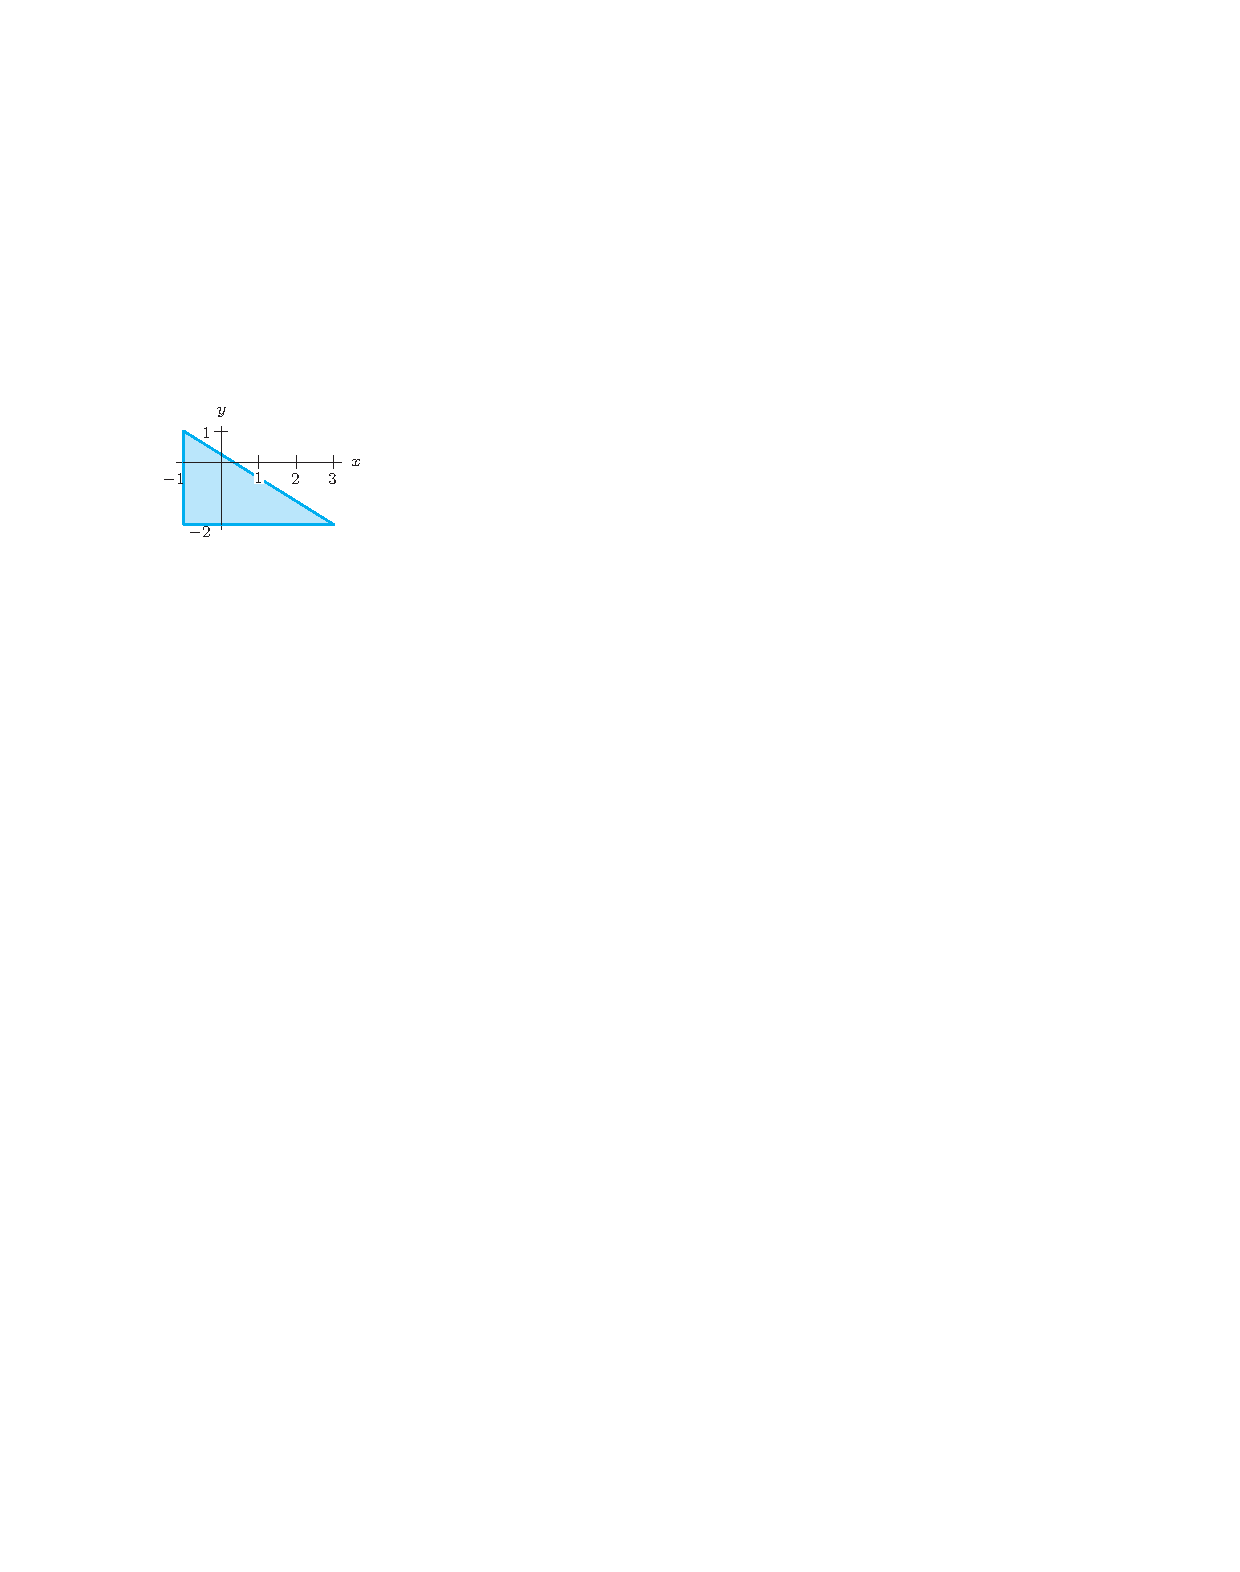
\includegraphics[scale=1.25]{pic5.pdf} $\textcolor{red}{\int_{-2}^{1} \int_{-1}^{-\frac{4}{3}y+\frac{1}{3}} f(x,y) \ dxdy = \int_{-1}^{3} \int_{-2}^{-\frac{3}{4}x+\frac{1}{4}} f(x,y) \ dydx}$
\end{enumerate}

\bigskip
\prob Compute the following iterated integrals. Sketch the region $R$ of integration.

\begin{enumerate}
\item $\displaystyle\int_0^2 \int_0^x e^{x^2} \ dy\ dx$

\bigskip
\textcolor{red}{
	\[\int_0^2 \int_0^x e^{x^2} \ dy\ dx = \int_0^2 e^{x^2}y\big|_0^x \ dy = \int_0^2 x e^{x^2} \ dx = \frac{1}{2} e^{x^2}\big|_0^2 = \frac{1}{2} e^4 - \frac{1}{2}.
	\]}
\bigskip

\item $\displaystyle\int_1^4 \int_{\sqrt{y}}^y x^2 y^3 \ dx \ dy$

\bigskip
\textcolor{red}{
	\[\int_1^4 \int_{\sqrt{y}}^y x^2 y^3 \ dx \ dy = \int_1^4 \frac{1}{3} x^3 y^3\big|^y_{\sqrt{y}} \ dy = \frac{1}{3} \int_1^4 (y^6 - y^{9/2}) \ dy =\frac{1}{3} \left[ \frac{y^7}{7} - \frac{2}{11} y^{11/2} \right]_1^4 =\frac{151555}{231}.
	\]}
\bigskip

\item $\displaystyle\int_1^5 \int_x^{2x} \sin{(x)} \ dy \ dx$

\bigskip
\textcolor{red}{
	\[\int_1^5 \int_x^{2x} \sin{(x)} \ dy \ dx = \int_1^5 y \sin{(x)}\big|_x^{2x} \ dx = \int_1^5 x\sin{(x)} \ dx = [-x\cos{(x)} + \sin{(x)}]_1^5 \approx  -2.68.
	\]}
\bigskip
\end{enumerate}

\vfill
\newpage
\prob Compute the following iterated integrals by reversing the order of integration.

\begin{enumerate}
\item $\displaystyle\int_0^2 \int_y^2 e^{x^2} \ dx \ dy$

\bigskip
\textcolor{red}{
	\[\int_0^2 \int_0^x e^{x^2} \ dy \ dx = \frac{1}{2} e^4 - \frac{1}{2}.
	\]}
\bigskip

\item $\displaystyle\int_0^1\int_{x^2}^1 \sqrt{y} \sin{(y)} \ dy dx$

\bigskip
\textcolor{red}{
\begin{align*}
\int_0^1\int_{0}^{\sqrt{y}} \sqrt{y} \sin{(y)} \ dx dy &= \int_0^1 x\sqrt{y} \sin{(y)} \big|_{0}^{\sqrt{y}} \ dx dy \\
&= \int_0^1 y \sin{(y)} \ dy \\
&= [ -y \cos{(y)} + \sin{(y)}]_0^1 \\
&= -\cos{(1)} + \sin{(1)}.
\end{align*}}
\bigskip
\end{enumerate}


\end{document}